可以将主机设备看作是独立设备一样,可以执行设备代码。总是有一些处理器运行主机程序,因此主机设备对我们的应用程序总是可用的。主机设备提供了一个保证,设备代码可以始终运行(不依赖加速器硬件),并有几个主要用途:\par

\begin{enumerate}
	\item \textbf{设备代码的开发}在没有任何加速器的系统上:常用的方式是在部署到HPC集群进行性能测试和优化之前,在本地系统上开发和测试设备代码。
	\item 使用非加速工具\textbf{调试设备代码}:加速工具通常通过公开底层API让开发者使用,这些API可能没有像主机端那样的调试工具。考虑到这一点,主机设备应该支持使用CPU开发,以便开发人员熟悉调试工具。
	\item \textbf{备份} 如果没有其他设备保证设备代码可以执行:主机端运行设备代码可能不以性能作为主要目标,因此需要考虑作一个功能性的备份,确保设备代码可以执行,但不一定对性能有所要求。
\end{enumerate}

主机设备在功能上类似于硬件加速器设备,可以绑定队列,可以执行设备代码。图2-8展示了主机设备中与其他加速器是对等的。它可以执行设备代码,就像CPU、GPU或FPGA一样,并且可以绑定一个或多个队列。\par

\hspace*{\fill} \par %插入空行
图2-8 主机设备可以像任何加速器一样执行设备代码
\begin{center}
	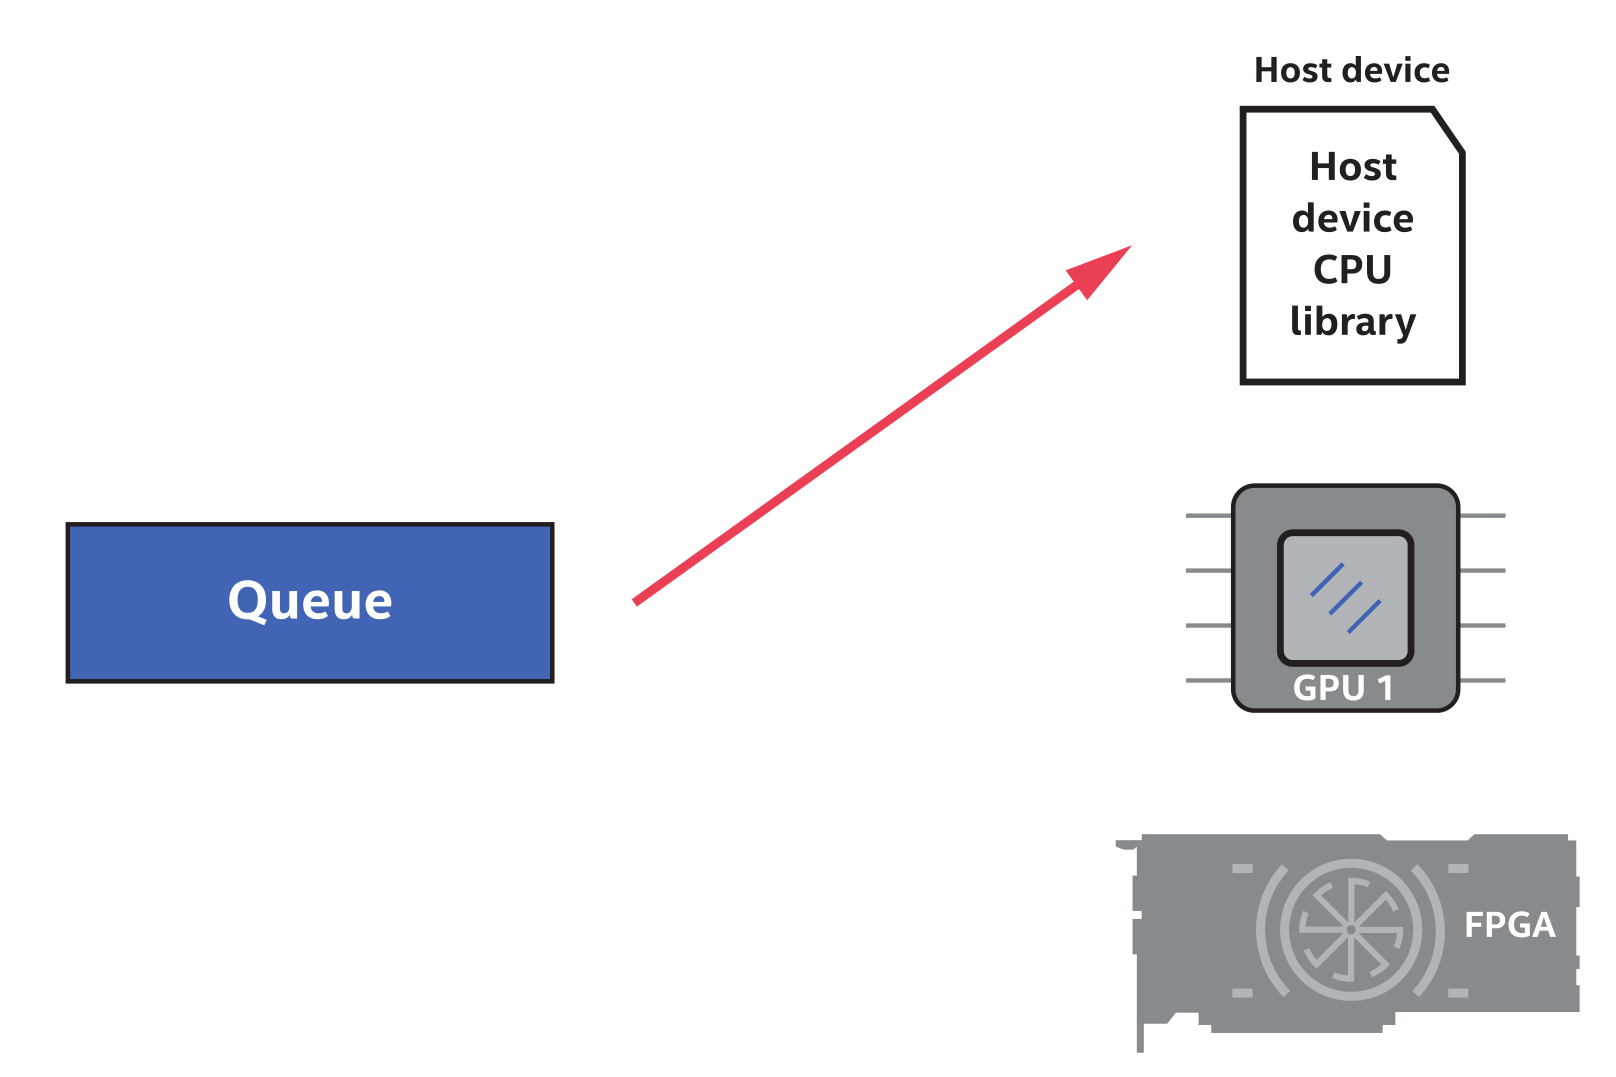
\includegraphics[width=0.8\textwidth]{content/chapter-2/images/6}
\end{center}

应用程序可以显式地将host\_selector传递给队列构造,来选择创建一个绑定到主机设备的队列,如图2-9所示。\par

\hspace*{\fill} \par %插入空行
图2-9 使用host\_selector选择主机设备
\begin{lstlisting}[caption={}]
#include <CL/sycl.hpp>
#include <iostream>
using namespace sycl;

int main() {
	// Create queue to use the host device explicitly
	queue Q{ host_selector{} };
	
	std::cout << "Selected device: " <<
	Q.get_device().get_info<info::device::name>() << "\n";
	std::cout << " -> Device vendor: " <<
	Q.get_device().get_info<info::device::vendor>() << "\n";
	
	return 0;
}

Possible Output:
Device: SYCL host device
\end{lstlisting}

即使没有特别的要求(例如,使用host\_selector),主机设备也可能会作为默认选项,如图2-7中的输出所示。\par

一些设备选择器类的变体,使我们可以很容易地指定一种类型的设备。host\_selector是这些选择器类的一个例子,我们将在接下来的几节中讨论其他的选择器类。\par






